\section{Глава 1. Задача оптимизации направленности фазированных антенных решеток}
\begin{frame}[plain, noframenumbering]
    \begin{center}
        \Huge
        Глава 1. Задача оптимизации направленности фазированных антенных решеток
    \end{center}
\end{frame}

\subsection{Постановка задачи}
\begin{frame}
    \frametitle{Постановка в комплексных числах}
    \begin{equation}
    f^{(l)}_{\Sigma} = \sum_{i=1}^{N}I_i \tilde{f}_i^{(l)}
    \label{eq:sumfield}
    \end{equation}

     \begin{equation}
        F = \sum_{l=1}^{2}\overline{f}_{\Sigma}^{(l)}f_{\Sigma}^{(l)}
        \label{eq:FPrimary}
    \end{equation}

        \begin{equation}
        F = \textbf{i}^{+}\textbf{Ai} \rightarrow \max
        \label{eq:F}
    \end{equation}

\vspace{2em}
    \textbf{Юрков А.С.:} Оптимизация возбуждения передающих фазированных антенных решеток декаметрового диапазона длин волн~// ОНИИП 2014.
\end{frame}

\begin{frame}
    \frametitle{Постановка в комплексных числах}
   \begin{equation}
        \begin{cases}
           \textbf{i}^{+}\textbf{Ai} \rightarrow \max,\\
           0 \leq \textbf{i}^{+}\textbf{B}^{(1)}\textbf{i} \leq 1, \\
           ...\\
           0 \leq \textbf{i}^{+}\textbf{B}^{(n)}\textbf{i} \leq 1,\\
           \textbf{i} \in \mathbb{C}^N\\
         \end{cases}
         \label{eq:task2}
    \end{equation}
%
где $n$ - число точек питания, на которые накладываются ограничения
%
    \begin{equation}
        \textbf{B}^{(k)} = \frac{1}{4P_{max}^{(k)}}(\textbf{Z}^{+}\mathcal{P}^{(k)} + \mathcal{P}^{(k)}\textbf{Z}) \, ,
    \end{equation}
%
$P_{max}^{(k)}$ - максимально допустимая мощность в $k$-й точке питания, $\mathcal{P}^{(k)}$ - матрицы-проекторы имеющие единственный ненулевой элемент $\mathcal{P}^{(k)}_{kk}=1$.

\vspace{2em}
    \textbf{Юрков А.С.:} Оптимизация возбуждения передающих фазированных антенных решеток декаметрового диапазона длин волн~// ОНИИП 2014.
\end{frame}

\begin{frame}
    \frametitle{Постановка в комплексных числах}
   \begin{enumerate}
  \item Все матрицы $\textbf{B}^{(k)}$ имеют не более чем два ненулевых собственных значения. Одно из собственных значений положительно,
  остальные отрицательные или нулевые.
  \item Матрицы $\textbf{A}$ и $\textbf{B}^{(k)}$ эрмитово-самосопряженные, то есть
  $a_{ij} = \overline{a}_{ji}$ для всех $i = \overline{1,N}, j = \overline{1,N}$.
  \item Матрица $\textbf{A}$ положительно полуопределена.
  \item Кроме того, из физических соображений вытекает, что матрица $\textbf{B}_{\Sigma}:= \sum_{k=1}^{n} \textbf{B}^{(k)}$
  положительно определена, так как суммарная активная мощность, поглощаемая пассивной цепью, не может быть отрицательной либо нулем,
  поскольку, часть энергии обязательно излучится.
\end{enumerate}

\vspace{2em}
    \textbf{Юрков А.С.:} Оптимизация возбуждения передающих фазированных антенных решеток декаметрового диапазона длин волн~// ОНИИП 2014.
\end{frame}

\begin{frame}
    \frametitle{Постановка в вещественных числах}
    \begin{equation}
        \begin{cases}
           \textbf{x}^{T}\textbf{Gx} \rightarrow \max,\\
           0 \leq \textbf{x}^{T}\textbf{H}^{(1)}\textbf{x} \leq 1,\\
           ...\\
           0 \leq \textbf{x}^{T}\textbf{H}^{(n)}\textbf{x} \leq 1,\\
          \textbf{x} \in \mathbb{R}^{2n}.\\
         \end{cases}
         \label{eq:task3}
    \end{equation}
Задача~(\ref{eq:task3}) имеет целевую функцию, заданную квадратичной формой с положительно полуопределенной матрицей~$\textbf{G}$. Каждое ограничение формулируется квадратичной формой, определенной симметричной матрицей~$\textbf{H}^{(k)}, k=\overline{1,n}$ с двумя парами идентичных собственных значений, два из которых положительны, а другие два отрицательны или равны нулю, все остальные собственные числа равны нулю.

\vspace{2em}


\footnotesize { \textbf{Ereemeev A.V., Tynin N.N., Yurkov A.S.:} Non-Convex Quadratic Programming Problems in Short Wave Antenna Array Optimization.~// MOTOR 2019 (11584) }
\end{frame}


\begin{frame}
    \frametitle{Постановка задачи}
    \begin{block}{Метод штрафных функций}
        \begin{equation}
               \textbf{x}^{T}\textbf{Gx} - r\cdot \sum_{k=1}^n
               \left( \min\left(0,\textbf{x}^{T}\textbf{H}^{(k)}\textbf{x}\right) +
               \min\left(0,1-\textbf{x}^{T}\textbf{H}^{(k)}\textbf{x}\right)\right)^{\alpha} \rightarrow
               \max
             \label{eq:task4}
        \end{equation}
    \end{block}

    \begin{block}{Фазовая симметрия}
        \begin{equation}
            \textbf{i} \to e^{~{j}\phi}\textbf{i}
             \label{eq:phase_sym}
        \end{equation}
    \end{block}
\end{frame}

\subsection{Верхняя оценка нормы допустимых решений}

\begin{frame}
    \frametitle{Верхняя оценка нормы допустимых решений}

    Если $\bf x$ удовлетворяет всем ограничениям задачи~(\ref{eq:task3}), то
$$
\sum_{k=1}^{n} {\bf x}^T {\bf H}^{(k)}  {\bf x} \le N.
$$
$${\bf H}_{\rm sum}:= \sum_{k=1}^{n} {\bf H}^{(k)}$$
$$\lambda_{\min} > 0$$
$$
\min\{{\bf z}^T {\bf H}_{\rm sum} {\bf z} \ : \ {\bf z}\in
\mathbb{R}^{2N}, \ ||{\bf z}|| =1\} = \lambda_{\min},
$$
$$
{\bf x}^T {\bf H}_{\rm sum} {\bf x} \ge ||{\bf x}||^2
\lambda_{\min}\ \
$$
\begin{equation} \label{eqn:bound}
||{\bf x}||\le \sqrt{\frac{N}{\lambda_{\min}}}.
\end{equation}

\vspace{2em}

\footnotesize { \textbf{Тюнин Н.Н.:} Задачи невыпуклого квадратичного программирования, связанные с оптимизацией фазированных антенных решеток~//Дискретный анализ и исследование операций, 2021, 28(3)}

\end{frame}

\subsection{Масштабирование решения в допустимую область}

\begin{frame}
    \frametitle{Масштабирование решения в допустимую область}

Если решение $\textbf{x}$ нарушает только ограничивающие неравенства задачи~(\ref{eq:task3}) вида $\textbf{x}^{T}\textbf{H}^{(k)}\textbf{x} \leq 1,$ то:

\begin{equation}
    {\bf x}': =\mu({\bf x})^{-1/2} {\bf x} ,
    \label{eq:scale}
\end{equation}
где $\mu({\bf x}):=\max_{k=\overline{1,n}} {\bf x}^T {\bf H}^{(k)}{\bf x}$.
\vspace{2em}

\footnotesize { \textbf{Тюнин Н.Н.:} Задачи невыпуклого квадратичного программирования, связанные с оптимизацией фазированных антенных решеток~//Дискретный анализ и исследование операций, 2021, 28(3)}

\end{frame}

\section{Глава 2. Структурные свойства задачи оптимизации направленности фазированных антенных решеток}
\begin{frame}[plain, noframenumbering]
    \begin{center}
        \Huge
        Глава 2. Структурные свойства задачи оптимизации направленности фазированных антенных решеток
    \end{center}
\end{frame}


%------------------------------------------------
\subsection{Вычислительный эксперимент}

\begin{frame}
    \frametitle{ Программный комплекс}

    \begin{figure}
    \centering
        \begin{minipage}[h]{1\linewidth}
                \center{\includegraphics[width=0.9\linewidth]{expi.png} }
        \end{minipage}
        \vspace{0.7em}
        \caption{Графический интерфейс программного комплекса}
        \label{ris:expi}
    \end{figure}

\end{frame}

\begin{frame}
    \frametitle{Сравнение результатов оптимизации градиентного подъема и решателя BARON}

\begin{table}[!h]
\centering
\caption{ Результаты оптимизации, полученные с помощью градиентного подъема и решателя BARON.}
\begin{tabular}{|c|c|c c|c c|}
    \hline
    \multirow{2}{*}{\textbf{Тип}} & \multirow{2}{*}{$\sqrt{\frac{N}{\lambda_{\min}}}$} & \multicolumn{2}{c}{\textbf{Град.}} & \multicolumn{2}{|c|}{\textbf{BARON}} \\
    & & \textbf{$\tilde{F}$} & \textbf{t, c} & \textbf{$\tilde{F}$} & \textbf{t, c} \\
    \hline
    ШВИ 2х2 & 13.6 & 138 & {0.054} & {139} & 0.12  \\
    ШВИ 3х3 & 22.5 & 576 & 0.93 & {581} & {0.34}  \\
    ШВД 2х2 & 21 & 460 & {0.13} & {464} & 0.27  \\
    ШВД 3х3 & 82.2 & 915 & 24.4 & {925} & {0.34}   \\
    СВД 2х2 & 44.7& 357 & 1.9 & {361} & {0.16}  \\
    СВД 3х3 & 641.9& 1138 & 25.6 & \textbf{1261} & {0.38} \\
    СВД 5х5 & $1.1\cdot10^{5}$ & 5318 & 1000 & 6716 & 1000 \\
    СВД' 2х2 & $2.3\cdot10^{4}$ & 233 & 2.52 & \textbf{253} & {0.25}  \\
    СВД' 3х3 & $6\cdot10^5$& 664 & 71 & \textbf{1153} & {1.48}  \\
    СВД' 5х5 & - & 1382 & 1000 & 33.5 & 217.94  \\
    Кольц. 8 & 87 & 217 & 8.06 & 218 & {0.23}  \\
    Кольц. 16          & 154 & 727 & 90.9 & 734 & {1.37}  \\
    \hline
\end{tabular}
\label{tab:results_0}
\end{table}
\end{frame}

\begin{frame}
    \frametitle{Статистический анализ}
    \begin{table}[!h]
    \centering
     \begin{tabular}{|l | l l | c c c | c c c|}
    \hline
    \textbf{ФАР} & \textbf{$M$} & \textbf{$M_{ne}$} & \textbf{$M_{f}$} & \textbf{$\mathcal{B}_{M_f}$} & \textbf{$\mathcal{L}_{M_f}$} & \textbf{$M_{y\approx0}$} & \textbf{$\mathcal{B}_{M_{y\approx0}}$} & \textbf{$\mathcal{L}_{M_{y\approx0}}$}\\
    \hline
    ШВИ 2x2 & 18368 & 4 & 1 & 1 & 1 & 4 & 4 & 4\\
    ШВД 2x2 & 7678  & 4 & 1 & 1 & 1 & 4 & 4 & 4\\
    СВД 2x2  & 523  & 1 & 1 & 1 & 1 & 1 & 1 & 1\\
    СВД 3x3  & 39  & 9 & 2 & 2 & 2 & 5 & 5 & 5\\
    СВД' 2x2  & 396  & 370 & 3 & 3 & 3 & 338 & 1000 & 1213\\
    СВД' 3x3  & 14  & 14 & 3 & 3 & 3 & 1 & 1 & 1\\
    ШВИ 3x3 & 1070  & 3 & 1 & 1 & 1 & 3 & 3 & 3 \\
    ШВД 3x3 & 41  & 4 & 4 & 4 & 4 & 1 & 1 & 1 \\
    Кольц. 8 & 124  & 9 & 2 & 2 & 2 & 9 & 9 & 9\\
    Кольц. 16 & 11  & 6 & 1 & 1 & 1& 6 & 6 & 6\\
    \hline
\end{tabular}
    \label{tab:structure2}
\end{table}
\end{frame}

\subsection{Область притяжения глобального оптимума}
\begin{frame}
    \frametitle{Область притяжения глобального оптимума}

    \begin{figure}
    \centering
        \begin{minipage}[h]{0.8\linewidth}
                \center{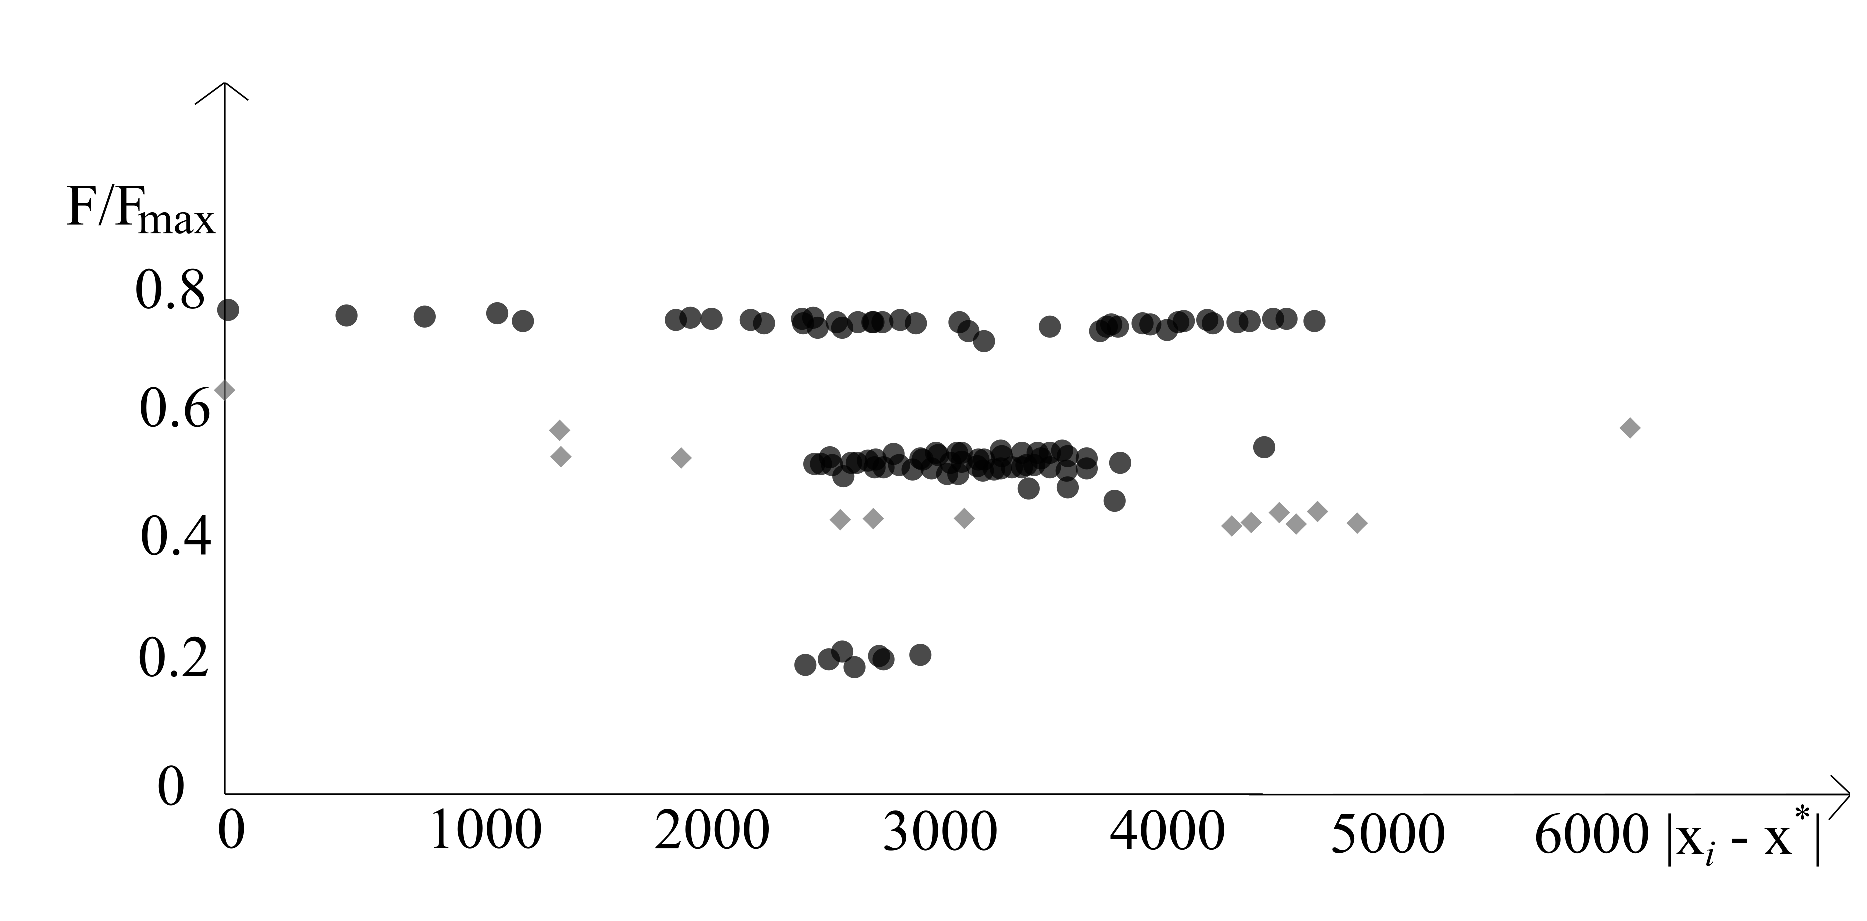
\includegraphics[width=0.9\linewidth]{fit_dist_2x2.eps} }
        \end{minipage}
        \vspace{0.7em}
        \caption{Зависимость качества локальных оптимумов от расстояния до глобального. Точками обозначены результаты для СВД'~2x2, ромбами - для СВД'~3x3.}
        \label{ris:fit_dist_2}
    \end{figure}

    Принимая на вход возмущенное порядка 0.5\% относительно нормы решения решателя BARON, градиентный подъем приводил к худшему решению.
\end{frame}

\subsection{Группы симметрий}

\begin{frame}
    \frametitle{Фазовая симметрия}
    $$\textbf{i} \to e^{~{j}\phi}\textbf{i}$$
    \vspace{2em}
    $$
    \hat{G}_1 =
    \left(
    \begin{array}{cccccccc}
      0 & 0 & 0 & . & -1 & 0 & 0 & . \\
      0 & 0 & 0 & . & 0 & -1 & 0 & . \\
      0 & 0 & 0 & . & 0 & 0 & -1 & . \\
      . & . & . & . & . & . & . & . \\
      1 & 0 & 0 & . & 0 & 0 & 0 & . \\
      0 & 1 & 0 & . & 0 & 0 & 0 & . \\
      0 & 0 & 1 & . & 0 & 0 & 0 & . \\
      . & . & . & . & . & . & . & .
    \end{array}
    \right)
    $$
\end{frame}

%------------------------------------------------

%\subsection{Дифференциальная эволюция}
%\begin{frame}
%    \frametitle{Дифференциальная эволюция}
%    // TODO: об алгоритма
%    \begin{itemize}
%      \item $v=v_{1}+f\cdot (v_{2}-v_{3}),$
%            где $v_1, v_2, v_3$ - случайные особи из текущей популяции, не равные друг другу.
%      \item Гибридный алгоритм с градиентным методом.
%    \end{itemize}
%\end{frame}

%------------------------------------------------

\section{Глава 3. Алгоритм дифференциальной эволюции для задачи оптимизации фазированных антенных решеток}
\begin{frame}[plain, noframenumbering]
    \begin{center}
        \Huge
        Глава 3. Алгоритм дифференциальной эволюции для задачи оптимизации фазированных антенных решеток
    \end{center}
\end{frame}
\begin{frame}
\subsection{Базовый вариант}
\frametitle{Базовый вариант}
\begin{figure}
\center{\includegraphics[width=0.55\linewidth]{233.png}}
\label{ris:ring}
\end{figure}
\end{frame}

\subsection{Гибридная реализация}
\begin{frame}
    \frametitle{Дифференциальная эволюция}
    \begin{itemize}
      \item Комбинация ДЭ и градиентного метода.
      \item Масштабирование в допустимую область.
      \item Фиксация фазы.
    \end{itemize}
\end{frame}

\begin{frame}
    \frametitle{Гибридная реализация ДЭ}

    \begin{flushleft}
    \small
    \verb"Пусть"
    $G_0$ -- \verb"номер поколения, когда было последнее улучшение рекорда,"\\
    %$D$ -- \verb"размер популяции,"\\
    $Grad(X)$ -- \verb"результат применения градиентного подъема с начальным решением "$X,$\\
    $X_G$ -- \verb"лучшая особь популяции на итерации "$G.$\\
    $\mbox{ }$\\

    \textit{Если} $G > D$ \textit{и} $G > 2 G_0,$ \textit{то положить} \\
    \leftskip=12pt
        $X' := Grad(X_G).$\\
        \textit{Если} $X'$ = $X_G,$ \textit{то} \verb"завершить выполнение алгоритма, выдать решение" $X_G.$\\
        \textit{Иначе положить} \\
        \leftskip=24pt
            $X_G := X',$\\
            $G_0 := G.$\\
            \leftskip=12pt
    \end{flushleft}
\end{frame}

\begin{frame}
    \frametitle{Адаптивный штраф}

    \begin{flushleft}
    \small
    \verb"Пусть"
    $G$ -- \verb"номер текущей итерации," \\
    $G_0$ -- \verb"номер итерации, на которой было получено улучшение рекорда,"\\
    $G_1$ -- \verb"номер итерации, на которой произошло предыдущее увеличение штрафа,"\\
    %$D$ -- \verb"размер популяции,"\\
    $r$ -- \verb"текущее значение штрафного коэффициента."\\
    $\mbox{ }$\\

    \textit{Если} $G > D$ \textit{и} $G > 1.5 G_0$ \textit{и} $G > 2 G_1,$  \textit{то положить} \\
    \leftskip=12pt
        $r := 2r$\\
        $G_1 := G.$\\
        \leftskip=0pt
    \end{flushleft}
\end{frame}

\subsection{Результаты вычислительного эксперимента}

\begin{frame}
    \frametitle{Результаты градиентного подъема, гибридного алгоритма ДЭ и BARON}
\begin{table}[!h]

\centering
\begin{tabular}{|c|c|c|cc|c c|}
    \hline
    \multirow{2}{*}{\textbf{Тип}} & \textbf{град. подъем} & \textbf{ДЭ} & \multicolumn{2}{|c|}{\textbf{BARON}} \\
    & \textbf{$\tilde{F}$} & \textbf{$\tilde{F}$} & \textbf{$\tilde{F}$} & \textbf{t, c}  \\
    \hline
    ШВИ 2х2         & ${138}$  & ${139}$   & 139    & 0.12      \\
    ШВИ 3х3         & ${576}$ & ${580}$   & 580    & 0.34       \\
    ШВД 2х2         & ${460}$ & ${463}$   & 463    & 0.27     \\
    ШВД 3х3         & ${915}$ & ${924}$   & 925    & 0.34        \\
    СВД 2х2        & ${357}$  & ${361}$   & 361    & 0.16         \\
    ШВИК 8-15(3:3) & ${217}$  & ${218}$   & 218    & 0.23       \\
    ШВИК 16-15(3:7)& ${727}$  & ${732}$   & 734    & 1.37     \\
    ШВДК 8-20      & ${1454}$  & ${1454}$  & 1455   & 2.78       \\
    ШВДК 8-30      & ${2422}$  & ${2422}$  & 2422   & 1.47     \\
    СВДК 8-25      & ${740}$  & ${740}$   & 740    & 0.23        \\
    СВДК 8-37      & ${1487}$  & ${1487}$  & 1487   & 0.23      \\
    \hline
\end{tabular}
\label{tab:results_de}
\end{table}
\end{frame}


\begin{frame}
    \frametitle{Результаты градиентного подъема, гибридного алгоритма ДЭ и BARON}
\begin{table}[!h]

\centering
\begin{tabular}{|c|c|c|cc|c c|}
    \hline
    \multirow{2}{*}{\textbf{Тип}} & \textbf{град. подъем} & \textbf{ДЭ} & \multicolumn{2}{|c|}{\textbf{BARON}} \\
    & \textbf{$\tilde{F}$} & \textbf{$\tilde{F}$} & \textbf{$\tilde{F}$} & \textbf{t, c}  \\
    \hline
    СВД 3х3        & ${1138}$ & 1163  & \textbf{1261}   & 0.38     \\
    СВД 5х5        & ${5318}$  & \textbf{7132}  & 6716   & 1000   \\
    СВД' 2х2       & ${233}$ & 198   & \textbf{253}    & 0.25         \\
    СВД' 3х3       & ${664}$ & 834   & \textbf{1153}   & 1.4          \\
    СВД' 5х5       & ${1382}$  & \textbf{2755}  & 33     & 217.94     \\
    ШВИК 8-15(2:3) & ${1536}$  & \textbf{1664}     & -   & 14.62     \\
    \hline
\end{tabular}
\label{tab:results_de}
\end{table}
\end{frame}

%------------------------------------------------
\begin{frame}
    \frametitle{Учет фазовой симметрии}
\begin{figure}
\center{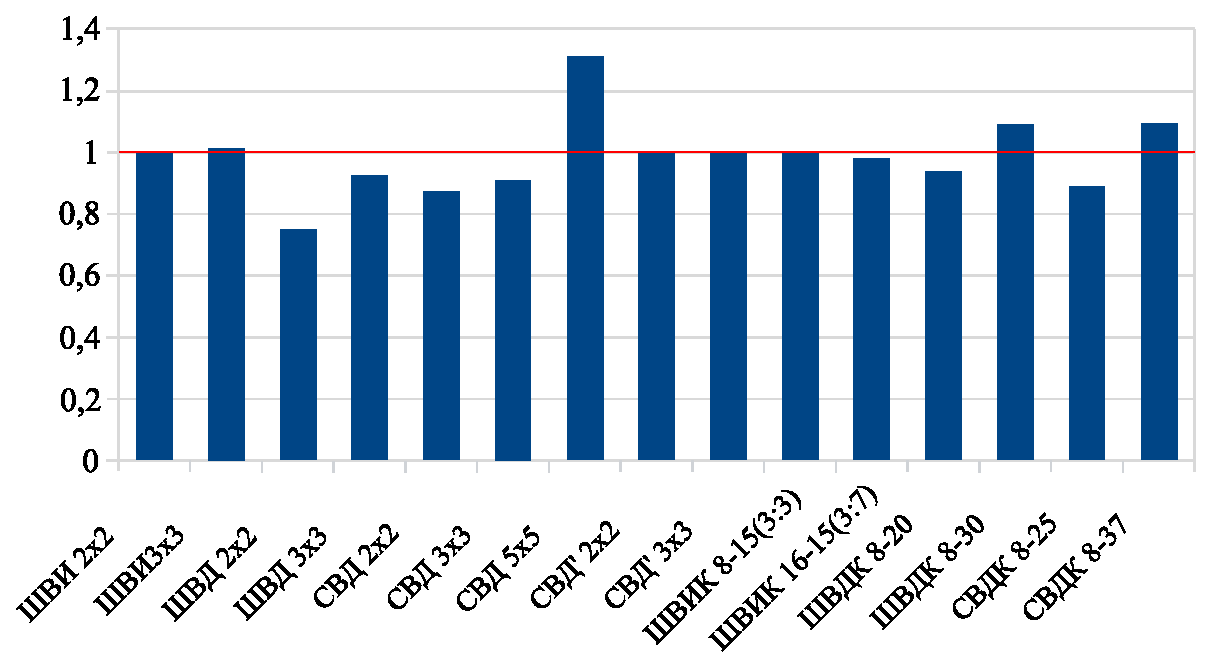
\includegraphics[width=0.8\linewidth]{ratio.eps}}
\caption{Отношение длительности вычислений с фиксацией первой координаты к исходной длительности вычислений}
\label{ris:ring}
\end{figure}
\end{frame}

\section{Глава 4. Возможности оптимизации фазированных антенных решеток в различных условиях}
\begin{frame}[plain, noframenumbering]
    \begin{center}
        \Huge
        Глава 4. Возможности оптимизации фазированных антенных решеток в различных условиях
    \end{center}
\end{frame}


\begin{frame}
    \frametitle{Кольцевые ФАР}
    \begin{figure}
    \center{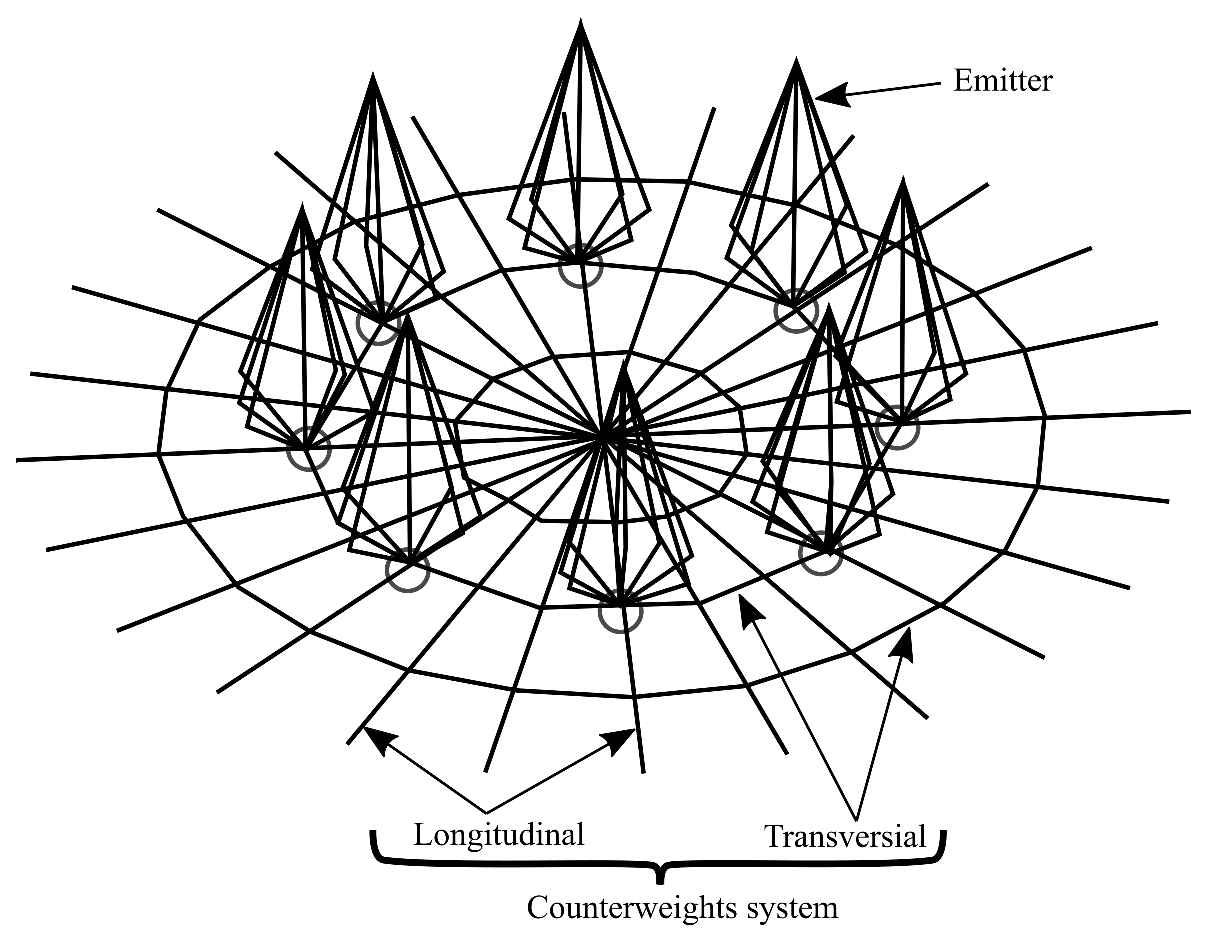
\includegraphics[width=0.6\linewidth]{r8.eps}}
    \caption{ФАР кольцевой структуры}
    \label{ris:rings}
    \end{figure}
\end{frame}

\subsection{Радиочастотные зависимости эффективности ФАР}

\begin{frame}
    \frametitle{Радиочастотные зависимости эффективности ФАР}
\begin{figure}
\begin{minipage}[h]{0.4\linewidth}
\center{\includegraphics[width=1\linewidth]{r8_1_25_5x7_marked.png}} а)
\end{minipage}
\hfill
\begin{minipage}[h]{0.4\linewidth}
\center{\includegraphics[width=1\linewidth]{r8_25_5x7_marked.png}} б)
\end{minipage}
\caption{Вертикальный план диаграммы направленности одиночного излучателя (a) и ФАР 5:7 (b) при 25МГц}
\label{ris:25MHz}
\end{figure}
\end{frame}


\subsection{Взаимное влияния излучателей}

\begin{frame}
    \frametitle{Взаимное влияние излучателей}
    \begin{figure}
    \begin{minipage}[h]{0.49\linewidth}
    \center{\includegraphics[width=1\linewidth]{r_bvd_20_results_h.png} \\ а)}
    \end{minipage}
    \hfill
    \begin{minipage}[h]{0.49\linewidth}
    \center{\includegraphics[width=1\linewidth]{r_bvd_20_results_v.png} \\ б)}
    \end{minipage}
    \caption{Горизонтальный (а) и вертикальный (б) план диаграммы направленности ШВД при расстоянии от центра излучателя до центра решетки 20 м. Пунктирной линией обозначено усиление одиночного излучателя, штрихпунктирной – простое фазирование, сплошной – решение задачи мат. программирования.}
    \label{pic:r_bvd_result_2}
    \end{figure}

\end{frame}